\begin{frame}
    \begin{hypothesis}[Riemannsche Hypothese]
        Abgesehen von den \glqq trivialen\grqq\ Nullstellen bei $s = -2n,\; n\in \N$ haben alle Nullstellen Realteil $\frac{1}{2}$.
    \end{hypothesis}
    \only<1>{
    \begin{figure}
        \begin{tikzpicture}
            \node[anchor=south west,inner sep=0] (image) at (0,0) {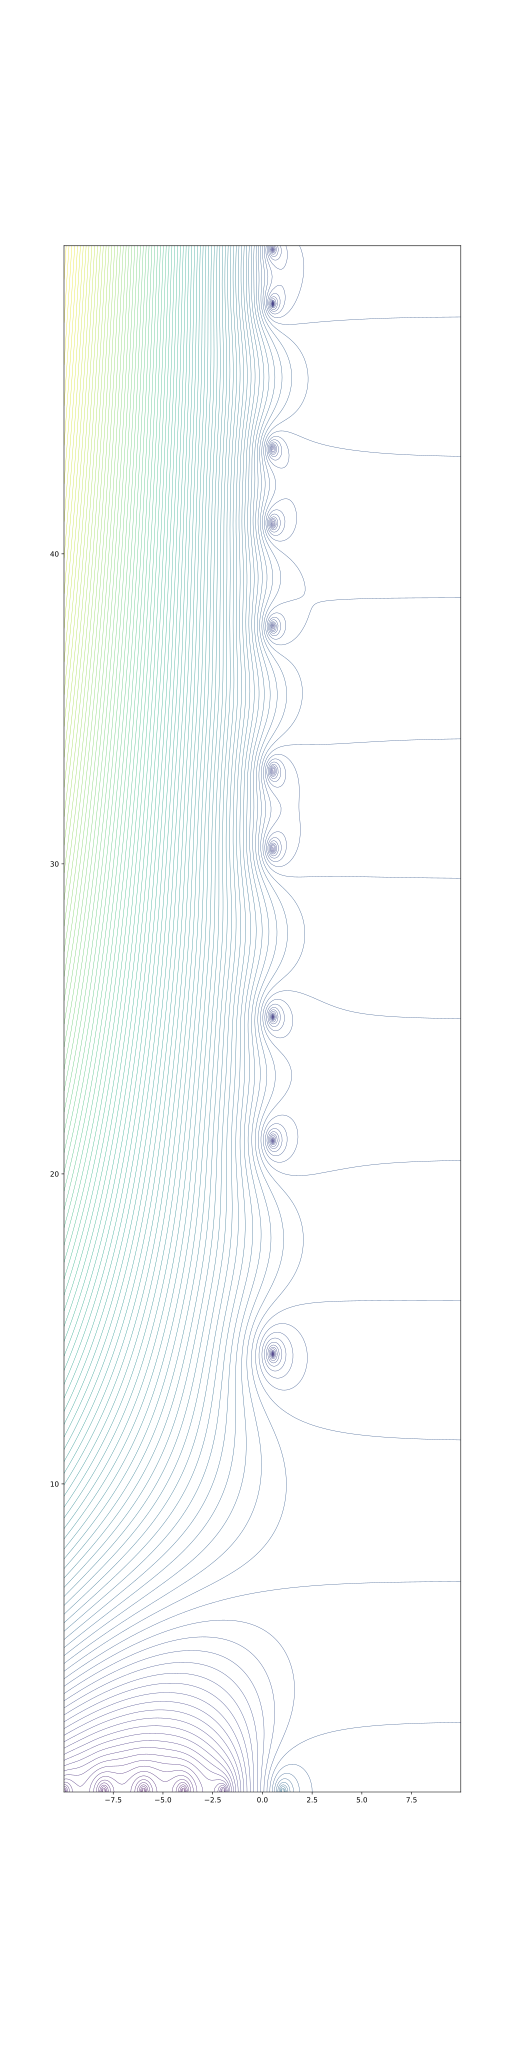
\includegraphics[width=0.8\textwidth, trim=231 46 195 44, clip]{figures/jupyter_zeros.pdf}};
            \begin{scope}[x={(image.south east)},y={(image.north west)}]
                %\draw[help lines,xstep=.1,ystep=.1] (0,0) grid (1,1);
                \foreach \y in {-10,-5,...,10} { 
                    \node [anchor=east] at (0,\y/20+0.5) {$\y$}; 
                    \draw (0,\y/20+0.5) -- (-1mm,\y/20+0.5);
                    }
                \foreach \x in {0,10,...,50} { 
                    \node [anchor=north] at (\x/50,0) {$\x$}; 
                    \draw (\x/50,0) -- (\x/50,-1mm);
                    }
                \node (ylabel) at (-.12,0.5) {$\operatorname{\Re s}$};
                \node (xlabel) at (0.5,-.25) {$\operatorname{\Im s}$};
                \draw[very thin] (0,0) rectangle (1,1);
            \end{scope}
        \end{tikzpicture}
        \caption{Absolutbetrag der $\zeta$-Funktion bei $\Re s = \frac{1}{2}$ von $\Im s = 0$ bis $\Im s = 50$}
    \end{figure}
    }
    \only<2>{
        \begin{center}
            \sagestr{output}
        \end{center}
    }
\end{frame}